% This version of CVPR template is provided by Ming-Ming Cheng.
% Please leave an issue if you found a bug:
% https://github.com/MCG-NKU/CVPR_Template.

\documentclass[final]{cvpr}

\usepackage{times}
\usepackage{epsfig}
\usepackage{graphicx}
\usepackage{amsmath}
\usepackage{amssymb}
\usepackage[numbers]{natbib}
\usepackage{notoccite}
\usepackage{subcaption}
\captionsetup{compatibility=false}

% Include other packages here, before hyperref.

% If you comment hyperref and then uncomment it, you should delete
% egpaper.aux before re-running latex.  (Or just hit 'q' on the first latex
% run, let it finish, and you should be clear).
\usepackage[pagebackref=true,breaklinks=true,colorlinks,bookmarks=false]{hyperref}


\def\cvprPaperID{34} % *** Enter the CVPR Paper ID here
\def\confYear{CVPR 2021}
%\setcounter{page}{4321} % For final version only


\begin{document}
	
	%%%%%%%%% TITLE
\title{Financial Sentiment Analysis\\
	\vspace{2mm}
	\large \normalfont Final Project Report}

\author{\textsc{Grisi} Clément\\
	École des Ponts ParisTech\\
	{\tt\small grisi.clement@gmail.com}
}

\maketitle

\begin{abstract}
	Financial and economic news is continuously monitored by financial market participants and plays an integral part of investment activity \cite{headlines}. The growing availability of financial texts in the wake of big data has challenged most organizations and led to an ever increasing demand for powerful analytical tools. Among them, sentiment analysis appears as an efficient method for extracting actionable insights from news headlines. \\
	\\Deep-learning based methods have shattered performance in many challenging natural language processing applications, including sentiment analysis. I take advantage of the present project to familiarize myself with all of these methods, including the recently introduced and popular Transformers \cite{transformer}, investigating their performance for financial sentiment analysis. My code will be publicly available at \small{\url{https://github.com/clementgr/sentiment-analysis}}
\end{abstract}

\section{Introduction}

Stock market movement prediction is a very challenging task due to the large amount of unforseen events that can cause stock prices to change. Today, stock trading involves much more than monitoring stock prices, as traders are generally looking for vast amount of market information, news and reports about the company they wish to buy stocks from. When new information becomes available, all actors in the economy update their positions and prices adjust accordingly.\\
\\
Financial texts have become more readily available due to the proliferation of postings on the Internet and the ever-increasing demands for market transparency. Dealing with this deluge of data has become increasingly challenging for business analysts. Be it daily news, financial reports, official company statements or tweets, financial texts have emerged as a precious source of information. They appear as a good proxy for the state of a company at a given period of time and carry important information that is of value in any financial decision.\\
\\
Under the efficient market hypothesis \cite{hypothesis}, “the efficiency of markets relies on the delivery of market information to the investors in a timely and correct manner". However, as the stream of market data continues to expand rapidly, manual analysis to derive actionable insights largely exceeds human capacities: perfectly informed and rational decisions is no longer attainable. In order to guide the attention of financial analysts over such continuous flow of data, it has become crucial to develop automated text analysis techniques capable of skimming through countless lines of text and picking up on relevant information.\\
\\
Natural language processing (NLP) techniques are particularly suited to make sense out of such unstructured data. Among these, sentiment analysis has ermerged as an important analytic tool for dealing with the current text boom \cite{headlines}. By revealing the latest trends in the public mood as reflected in the media, sentiment analysis provides clues for making better decisions in chaotic financial markets. Though NLP has traditionally employed machine learning models for sentiment analysis, the ever increasing amount of textual data available has favored the emergence of deep learning based approaches, which will be the focus of this project.

\section{Problem Definition}

Sentiment analysis is the task of extracting sentiments or opinions of people from written language \cite{liu_2015}. Though it ranges from detecting emotions (e.g., fear, happiness), to sarcasm and intent (e.g., complaints, feedback), I will focus on its simplest form, that is classifying text as positive, negative or neutral.\\
\\
Given the complexity of human language, sentiment analysis is far from trivial. Financial sentiment analysis is even more challenging due to the use of domain-specific language and the unavailability of large annotated datasets. Let's consider a simple -- yet interesting -- example to better grasp the possible difficulties of the task:

\vspace{2mm}

\begin{quote}
	\centering
	\textit{Shares of food delivery companies surged despite the catastrophic impact of coronavirus on global markets.}
\end{quote}

\vspace{2mm}

\noindent 
The above statement contains a clear positive message about food delivery companies, together with a negative message about global markets. It is difficult for computers to extract this positive message because they would have to crack the financial context and understand what is positive and what is negative from the financial point of view.\\
\\
Due to the numerous challenges it involves, sentiment analysis in finance has become an important research topic \cite{financial_sentiment-1,financial_sentiment-2,financial_sentiment-3,financial_sentiment-4,financial_sentiment-5}. In spite of being highly unstructured, textual data is certainly not random sequences of characters. Researchers have long treated words as atomic units, simply representing them as indices in a vocabulary. However, such a representation of words comes short in analyzing deeper semantic meaning of a given text: it completely disregards grammar, and doesn't provide any notion of similarity between words. Hence, NLP gradually shifted from discrete word counting to continuous vector representations of words. Deep learning based approaches, which allow for complex feature extraction, location identification, and order information, have greatly contributed to this transition.

\section{Related Work}

Previous research conducted on sentiment analysis can be divided into two groups: 1) machine learning methods with features extracted from text based on word counting \cite{ml-1, ml-2, tfidf}, 2) deep learning approaches leveraging distributed representations of words \cite{dl-1, dl-2, dl-3}.\\
\\
A survey by Loughran and McDonald \cite{loughran} recapitulates the recent works on financial text analysis using machine learning with (discrete) bag-of-words approach and lexicon-based methods. For example, the same authors created an expert annotated dictionnary of positive, negative, and neutral financial terms, which enabled them to measure the sentiment of a sentence by counting words with a specific dictionary value. Another important example is \cite{naivebayes}, which compares various machine-learning binary classifiers to predict tweets sentiments. They show that the SVM classifier is more accurate compared to Decision Trees and Naïve Bayes classifier.\\
\noindent
One of the first papers that used deep learning methods for financial sentiment analysis was \cite{kraus}. Authors apply an long short-term memory (LSTM) neural network to predict stock-market movements from company announcements and show that method to be more accurate than traditional machine learning approaches. Several other works confirm the efficiency of deep learning models for financial sentiment analysis, including recurrent neural network (RNN) \cite{rnn-1, rnn-2}, convolutional neural networks (CNN) \cite{cnn-1, cnn-2} and attention mechanism \cite{att-1}. Before Transfromers were introduced, the state-of-the-art on the Financial PhraseBank dataset\footnote{this is the dataset I have used for this project} was held by an LSTM \cite{sota_lstm}.\\
\\
The success of deep learning based methods in NLP relies to a large extent on the introduction and improvement of text representation methods, such as word encoders \cite{word2vec, glove, elmo}. These convert words into distributed representations encoding the semantic information contained in words and sentences, which is crucial for sentiment analysis. The current state-of-the-art on the Financial PhraseBank dataset is held by \cite{FinBERT}, who use a Transformer-based architecture.

%	Deep-learning methods use a cascade of multiple layers of non-linear processing units for complex feature extraction and transformation. Each successive layer uses the output from the previous layer as input, thus extracting complex features which in many cases can be useful for generating learning patterns and relationships beyond immediate neighbors in the sequence. 

\section{Methodology}

\subsection{Dataset}

The dataset used is Financial PhraseBank \cite{malo}, a public dataset for financial sentiment classification. It consists of $4845$ english sentences selected randomly from financial news found on LexisNexis database. Annotators with background in finance were asked to label these sentences according to how they think the information contained might affect the mentioned company stock price: positive, negative \& neutral. Figure \ref{fig:label_distribution} shows the label distribution in the whole dataset. 

\begin{figure}[h!]
	\centering
	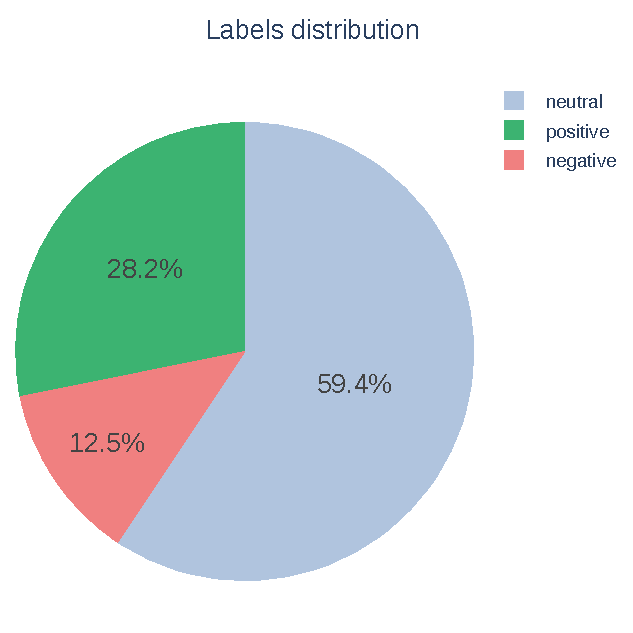
\includegraphics[width=5.8cm]{fig/label_distribution.pdf}
	\caption{Financial PhraseBank Label Distribution}
	\label{fig:label_distribution}
\end{figure}

In order to be able to compare to results reported on this dataset in the litterature, I used the same train/val/test split as performed by the authors of \cite{FinBERT}: they set aside $20\%$ of all sentences as test ($970$) and $20\%$ of the remaining as validation set ($388$). In the end, the training set includes $3488$ examples. Figure \ref{fig:sub_abel_distribution} shows the label distribution for each subset: we see that they all follow the distribution of the full dataset, which is a desirable property.

\begin{figure}[h!]
	\centering
	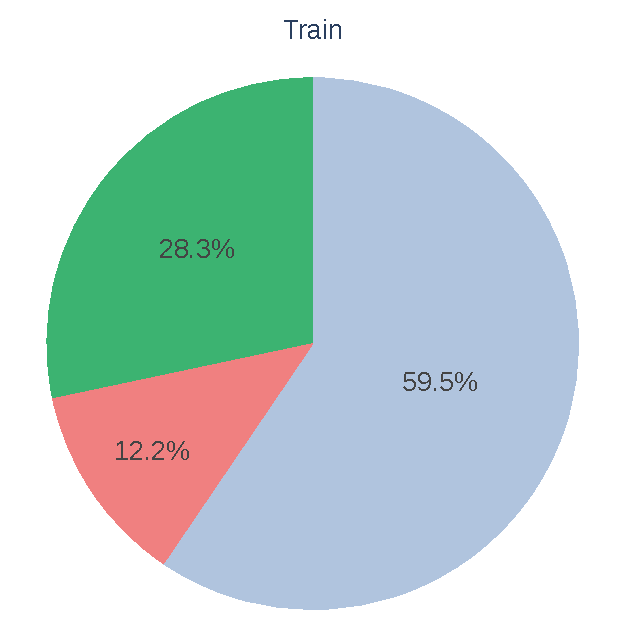
\includegraphics[width=4.0cm]{fig/label_distribution_train.pdf}
	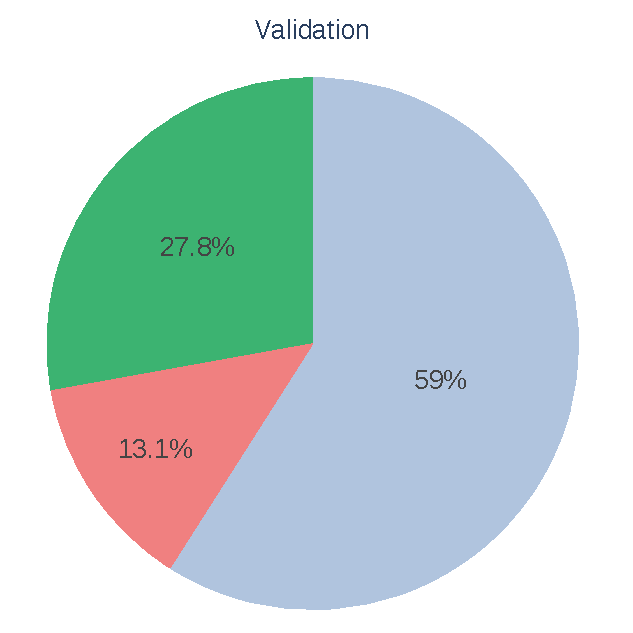
\includegraphics[width=4.0cm]{fig/label_distribution_val.pdf}
	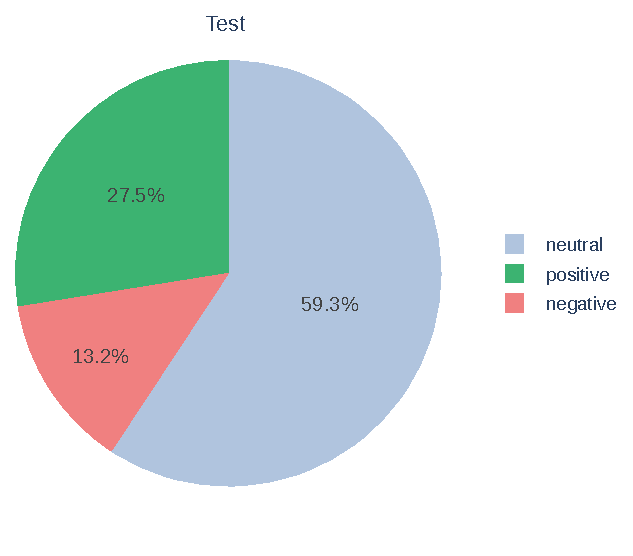
\includegraphics[width=4.9cm]{fig/label_distribution_test.pdf}
	\caption{Train / Validation / Test Label Distributions}
	\label{fig:sub_abel_distribution}
\end{figure}

\subsection{Evaluation Metrics}

To evaluate the performance of the various sentiment classification models I trained, I report three metrics: accuracy, micro and macro F1 average. Macro F1 average treats all classes equally as it computes the metric independently for each class and then take the average. Micro F1 average will aggregate the contributions of all classes to compute the average F1 score. In a multi-class classification setup, micro average is preferable in case of class imbalance. Since the Financial PhraseBank suffers from label imbalance (almost $60$\% of all sentences are neutral), I will base the comparison of models on this particular metric.

%	To bring stability to my results, I used $5$-fold cross validation in most of the deep learning experiments.

%	 I weight cross entropy loss with square root of inverse frequency rate. For example if a label constitutes $16$\% of the all examples, I weight the loss attributed to that label by $2.5$. 

\subsection{Text Pre-processing}

Financial headlines, similar to other real world text data, are likely to be inconsistent, incomplete and contain errors. Hence, to prepare the data, I perform initial pre-processing, starting with tokenization. Once the text tokenized, I remove stopwords and punctuation, which are required for correct grammar but add little to sentiment or context analysis. I used the stopwords corpus from NLTK for stopwords removal. Eventully, I lemmatized (i.e. grouped together the inflected forms of a word so they can be analysed as a single item) sentences using the WordNet Lemmatizer. After this initial filtering, I obtain the distributions of the number of words per sentence for the training set and the validation set (Figure \ref{fig:stopwords}).

\begin{figure*}[t!]
	\centering
	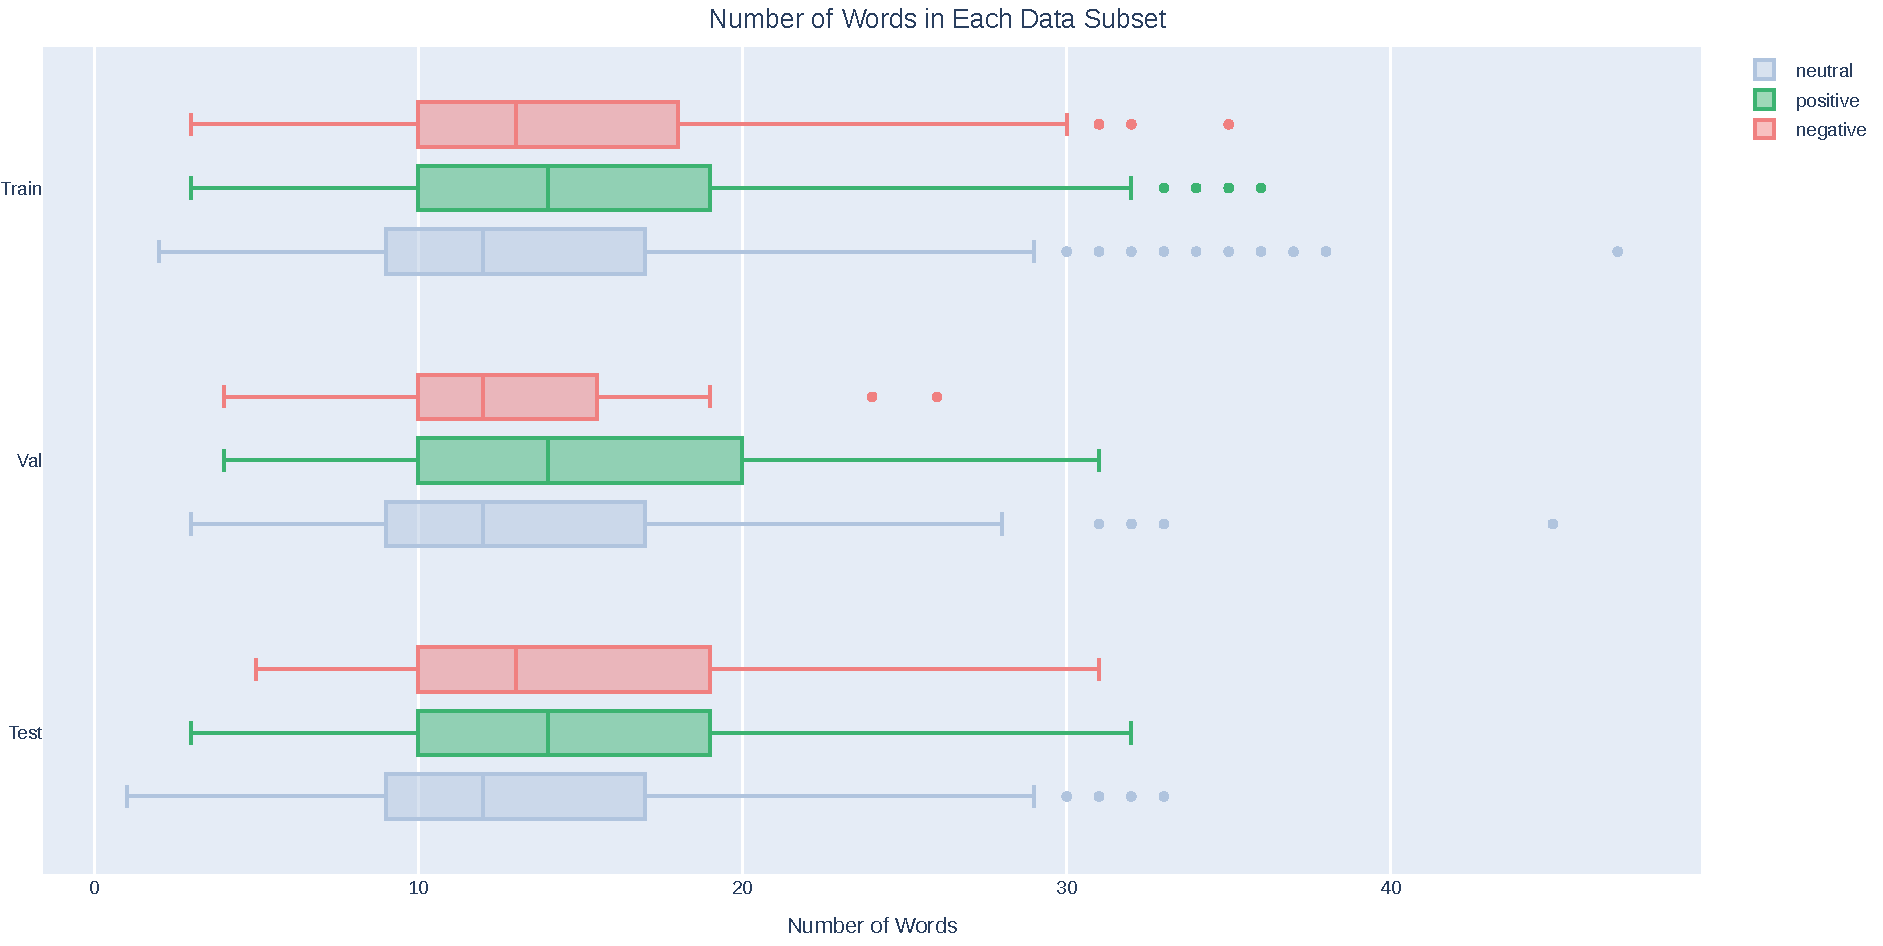
\includegraphics[width=1.05\textwidth]{fig/number_of_words.pdf}
	\caption{Boxplot of the Number of Words in Train / Validation / Test Subsets}
	\label{fig:stopwords}
\end{figure*}

%	\vspace{4mm}
%	\noindent
%	Interestingly, I found that removing stopwords using the NLTK stopwords corpus significantly decreases the accuracy of classification. This is probably due to the fact that the stopwords corpus from NLTK includes words that could be very useful for financial sentiment analysis (e.g. “up”, “down”, “below” or “above”). It would be interesting to consider a more restrictive list of stopwords for financial sentiment analysis

\subsection{Text Representation}

In order to be able to process text data with a computer, one first need to encode words in a numeric form. To date, there are two main families of methods mapping words to vectors of real numbers. Statistical models offer simple categorical encodings. Yet, they treat all words as independent entities and are unable to provide any notion of similarity between words. With deep learning encoders, word embeddings become contextualized: they capture complex relationships, efficiently encoding semantic information that might be relevant to the task at hand.

\subsubsection{Statistical Models}

A very basic way to numerically represent words is through the count vectorizing (CV) method (also known as one-hot encoding). It simply consists of assigning each word its index in the vocabulary of unique words present in a text, and produces sparse vectors the size of the vocabulary. In spite of being fast to compute and relatively robust, this approach has some drawbacks. Such a representation suffers from the inability to provide any meaningful notion of similarity between words: in the resulting vector space, each word vector is orthogonal and equidistant to the others. By simply relying on counting, it also gives more weight to general, frequent words such as “the”, “and”, or “but”, which barely add meaningful information.  As a result, important text features tend to vanish.\\
\\
Term frequency - inverse document frequency (TF-IDF) is another statistical algorithm which addresses the feature-vanishing issue of count vectorizing algorithms. By re-weighting the count frequencies of words according to their number of appearances in the text, frequent words are given smaller significance.\\
\\
Both of these methods suffer from the inability to capture the contextual information of a sentence. To overcome this, researchers have developed neural probabilistic models to convert discrete words into high-dimensional dense vectors capable of encoding the rich semantic information contained in text data.

\subsubsection{Word Encoders}

Sentiment analysis requires detailed semantic knowledge that is not provided by the statistical features extracted with CV and TF-IDF. Based on the distributional hypothesis, which assume that the complete meaning of a word is always contextual, researchers came up with word encoders. Word encoders classify words appearing in the same context as semantically similar to one another, hence assigning similar vectors to them. This approach, based on the principle famously summarised by J.R. Firth as “\textit{you shall know a word by the company it keeps}”, establishes a new area of research called distributional semantics. Let's present three of the most popular word emcoding techniques, namely Word2Vec \cite{word2vec}, GloVe \cite{glove} and ELMo \cite{elmo}.\\
\\
Word2Vec \cite{word2vec}, introduced in 2013 by a team of researchers at Google, is considered to be the staring point of the still ongoing revolution in NLP. It computes continuous vector representations of words using two model architectures: Continuous Bag-of-Words (CBOW) and Skip-Gram (SG). The CBOW architecture predicts a center word from its (bag of) context words, while the SG architecture predicts context words given a center word. The authors show the effectiveness of both word encoding methods experimentally using several NLP applications, including sentiment analysis.\\
\\
GloVe \cite{glove} was introduced in 2014 by a team of researchers at Stanford University. Based on a solid mathematical approach, GloVe overcomes the drawbacks of Word2Vec, ultimately improving the generated word embeddings. It emphasizes the importance of considering the co-occurrence probabilities between the words rather than single word occurrence probabilities themselves. GloVe is widely used as a word encoder for sentiment analysis.\\
\\
Word2Vec and GloVe produce static embeddings for each words. This one-to-one mapping is, in many cases, inappropriatem qs words often have different meaning depending on the sentence they are used in. To account for this, a team of researchers at the Allen Institute introduced in 2018 an advanced word encoder called ELMo (Embeddings from Language Models) \cite{elmo}. Instead of using a fixed embedding for each word, ELMo looks at the entire sentence before assigning each word in it an embedding. This is achieved leveraging a deep bidirectional language model, pre-trained on large corpora of textual data. The resulting encoder produces \textit{contextual} word embeddings based on the whole context in which a word is used.\\
\\
Transformers \cite{transformer}, introduced in 2018, build on top of a number of these clever ideas. The release of BERT (Bidirectional Encoder Representations from Transformers) \cite{BERT}, an event described as marking the beginning of a new era in natural language processing, brought efficient word encoding to another level. I give more details on the inner working of Transformers in Section \ref{sec:transformers}.

\section{Results}

\subsection{Baseline Method}

The idea was to have reference results against which I could compare the performances of the more sophisticated models I would later develop. I decided to go with a simple baseline approach: fit a logistic regression on the one-hot encoded sentences. I also trained two other logistic regressions, one using GloVe embeddings ($100$-dimensional vectors), and another one using the embeddings extracted with a pre-trained version of BERT ($768$-dimensional vectors). In each experiment, the sentence embeddings simply consists of the sum of its word embeddings (Table \ref{tab:logistic_regression}). Interestingly, the one-hot encoded vectors seemed to produce better results. I haven't found an explaination to this observation.

\begin{table}[h!]
	\begin{center}
		\begin{tabular}{ l c c c  } 
			\hline
			\\ [-1.7mm] 
			Input & Accuracy & macro F1 & micro F1 \\ [0.7mm] 
			\hline
			\\ [-1.5mm] 
			1-hot encodings & 0.76 & 0.69 & \textbf{0.76} \\
			GloVe embeddings & 0.59 & 0.25 & 0.44 \\
			BERT embeddings & 0.72 & 0.68 & 0.72 \\[0.5mm] 
			\hline
			\\ [-0.9mm] 
		\end{tabular}
		\caption{Baseline Results}
		\label{tab:logistic_regression}
	\end{center}
\end{table}

\vspace{-5mm}

\subsection{Recurent Neural Networks}

Recurent Neural Networks (RNNs) \cite{rnn-original} are one of the primary architectures when it comes to dealing with sequencial data, such as text (a sentence is simply a sequence of words). They are particularly convenient as they can process inputs of any length and their size doesn’t increase for longer inputs. Through the use of hidden states and shared weights, they were designed such that the computation for step \textit{t} can use information from many steps back (at least in theory). In practive, however, they suffer from long term dependencies issues: the network has difficulties accessing information many steps back. This usually causes the gradient to vanish when backpropagating through earlier layers and the network to “forget" about past information. As such, RNNs are better at learning sequential recency than syntactic recency.\\
\\
Table \ref{tab:rnn} summarizes the results obained when training RNNs in four different configurations. I first trained a plain 1-layer deep RNN on GloVe embeddings. It achieved $0.60$ micro F1 average on the held out test set. Then, I trained a bidirectional RNN. It simply consists of putting two independent RNNs together: one is fed the input sequence in normal time order, while the other one is fed the same sequence in reverse time order. Both RNNs produce a sequence of hidden states, which are concatenated input-wise: concatenated hidden states rely on both left and right context. This is particularly valuable when trying to do sentiment analysis. Indeed, consider the following sentence: 

\vspace{2mm}

\begin{quote}
	\centering
	\textit{The company released its latest results: these were terribly exciting !}
\end{quote}

\vspace{2mm}

We can regard the hidden state corresponding to the word \textit{terribly} as a representation of this word in the context of this sentence. In the case of a plain RNN, this contextualized representation only contains information from the \textit{left} context. Yet, the \textit{right} context, which is the word \textit{exciting}, modifies the true meaning of the word \textit{terrible}, from negative to positive. This motivates why we might want to have information from both left and right when computing the contextualized representations of words in a sentence, which is precisely the purpose of bidirectional RNNs. Switching from unidirectional to bidirectional slightly improves the miro F1 average (from $0.60$ to $0.62$). The two other configurations simply consists of stacking 3 RNNs (be them plain or bidirectionnal) on top of each other. The best results were achived when training the 3-layer deep, bidirectional RNN

\begin{table}[h!]
	\begin{center}
		\begin{tabular}{ l c c c  } 
			\hline
			\\ [-1.7mm] 
			Model & Accuracy & macro F1 & micro F1 \\ [0.7mm] 
			\hline
			\\ [-1.5mm] 
			RNN & 0.67 & 0.47 & 0.60 \\
			bidir. RNN & 0.65 & 0.50 & 0.62 \\
			stacked RNN & 0.67 & 0.44 & 0.61 \\
			stacked bidir. RNN & 0.68 & 0.53 & \textbf{0.64} \\ [0.5mm] 
			\hline
			\\ [-0.9mm] 
		\end{tabular}
		\caption{RNN Results}
		\label{tab:rnn}
	\end{center}
\end{table}

\vspace{-4mm}

Several extensions of the classic RNN architecture have been designed to increase the memory capacity of the network along with the features extraction capacity. I will explore two of them: long short-term memory (LSTM) \cite{lstm-original}, and gated recurent units (GRU) \cite{gru-original}.

\subsection{Long Short-Term Memory}

LSTMs are a type of recurrent neural network that allows long-term dependencies in a sequence to persist in the network by using “forget" and “update" gates. At each step \textit{t}, we do not only have a hidden state $h_t$, but also a cell state $c_t$, which stores long-term information. LSTMs can erase, write and read information from the cell: the selection of which information is erased / written / read is controlled by three corresponding dynamic\footnote{dynamic means their value is computed based on the current context} gates. Mathematically, the cell can be seen as a route allowing the gradient to flow through the network without vanishing.\\
\\
Table \ref{tab:lstm} summarizes the results obained when training LSTMs in four different configurations, each time feeding GloVe embeddings. Here again, there is no significant difference between each configuration, though the 3-layer deep, bidirectionnal LSTM performs best.

\begin{table}[h!]
	\begin{center}
		\begin{tabular}{ l c c c  } 
			\hline
			\\ [-1.7mm] 
			Model & Accuracy & macro F1 & micro F1 \\ [0.7mm] 
			\hline
			\\ [-1.5mm] 
			LSTM & 0.76 & 0.71 & 0.76 \\
			bidir. LSTM & 0.75 & 0.72 & 0.76 \\
			stacked LSTM & 0.76 & 0.71 & 0.76\\
			stacked bidir. LSTM & 0.77 & 0.73 & \textbf{0.77} \\ [0.5mm] 
			\hline
			\\ [-2.9mm] 
		\end{tabular}
		\caption{LSTM Results}
		\label{tab:lstm}
	\end{center}
\end{table}

\vspace{-3mm}

\subsection{Gated Recurent Units}

GRUs are a simpler alternative to LSTMs, as there is no cell state involved. This architecture introduces an update gate which determines the quantity of information to keep from the past as well as a reset gate which sets the quantity of information to forget. Having fewer parameters, they are faster to train. Table \ref{tab:gru} summarizes the results obained when training GRUs in four different configurations, feeding GloVe embeddings. Once again, there is no significant difference between each configuration, though the 3-layer deep, bidirectionnal GRU performs best.

\begin{table}[h!]
	\begin{center}
		\begin{tabular}{ l c c c  } 
			\hline
			\\ [-1.7mm] 
			Model & Accuracy & macro F1 & micro F1 \\ [0.7mm] 
			\hline
			\\ [-1.5mm] 
			GRU & 0.77 & 0.74 & 0.77 \\
			bidir. GRU & 0.77 & 0.73 & 0.77 \\
			stacked GRU & 0.78 & 0.73 & 0.77 \\
			stacked bidir. GRU & 0.78 & 0.75 & \textbf{0.78} \\ [0.5mm] 
			\hline
			\\ [-2.9mm] 
		\end{tabular}
		\caption{GRU Results}
		\label{tab:gru}
	\end{center}
\end{table}

\vspace{-4mm}

In spite of solving the vanishing gradient issue, LSTMs and GRUs still suffer from a major drawback: recurrent computation is slow. The sequential nature of these architectures precludes parallelization within training examples which becomes critical at longer sequence length as memory constraints limit batching across examples. Transformers \cite{transformer} were introduced with the purpose to avoid recursion in order to allow parallel computation, as well as to reduce the observed drop in performances due to long-term dependencies.\\
\\
Remark: I wish I had had time to use ELMo embeddings as well to assess the impact switching from static to dynamic word embeddings has on model's performances, but I didn't have time for this.


\subsection{Transformers}\label{sec:transformers}

The Transformer \cite{transformer} is an attention-based architecture for modeling sequential information, that is an alternative to recurrent neural networks. It was proposed as a sequence-to-sequence model, therefore including encoder and decoder mechanisms. When performing sentence classification such as sentiment analysis, only on the encoder part is used. As clearly explained in \cite{FinBERT}, “\textit{the encoder consists of multiple identical Transformer layers. Each layer has a multi-headed self-attention layer and a fully connected feed-forward network. For one self-attention layer, three mappings from} {[token]} \textit{embeddings (key, query and value) are learned. Using each token’s key and all tokens’ query vectors, a similarity score is calculated with dot product. These scores are used to weight the value vectors to arrive at the new representation of the token. With the multi-headed self-attention, these layers are concatenated together, so that the sequence can be evaluated from varying “perspectives". Then the resulted vectors go through fully connected networks with shared parameters.}"\\
\\	
In 2018, researchers leveraged the transformer architecture to introduce a revolutionary language representation model, called BERT (Bidirectional Encoder Representations from Transformers) \cite{BERT}. BERT relies on the unsupervised learning approach to pre-train deep bidirectional representations from large unlabeled text corpora by using two new pre-training objectives: 1) masked language modelling, which consists of predicting randomly masked words in a sentence, and 2) next sentence prediction, which consist of predicting whether two given sentences actually follow each other. In both case, the input sequence is represented with token and positional embeddings, the later being used to remember the order of words in the sequence. Two speicial tokens denoted by [CLS] and [SEP] are added to the beginning and end of the sequence respectively.\\
\\
The most straight-forward way to use BERT is to use it to classify a single piece of text, which is precisely the ultimate goal of sentiment analysis. Table \ref{tab:bert} shows the results obtained when training BERT from scratch vs. when fine-tuning a pre-trained version of BERT on the Financial PhraseBank dataset. 

\begin{table}[h!]
	\begin{center}
		\begin{tabular}{ l c c c  } 
			\hline
			\\ [-1.7mm] 
			Configuration & Accuracy & macro F1 & micro F1 \\ [0.7mm] 
			\hline
			\\ [-1.5mm] 
			BERT (from scratch) & 0.67 & 0.55 & 0.66 \\
			BERT (pre-trained) & 0.85 & 0.83 & \textbf{0.85} \\ [0.5mm] 
			\hline
			\\ [-2.6mm] 
		\end{tabular}
		\caption{BERT Results}
		\label{tab:bert}
	\end{center}
\end{table}

\vspace{-2mm}	

These results show the effectiveness of pre-trained language models, as the pre-trained BERT beats all previous models by a large margin. The BERT model trained from scratch performs poorly due to the relatively small size of the dataset I am using and the important number of parameters that such a model has to learn.

\subsection{Error Analysis}

Analysing where a given model successfully classsifies sentiments or fails to do so can reveal important information, either about the overall behavior -- or tendency -- of this model, or more general information such as the quality of the labels in the dataset. Figure \ref{fig:cms} shows the confusion matrices of the best performing GRU and BERT models. Even though BERT is more accurate, we see that in both case, the main source of error comes from the positive vs. neutral sentences. Explicitely looking at some of the sentences where both models failed to predict the true sentiment might give some clues about the reasons behind these mistakes.

\begin{figure}[h!]
	\begin{subfigure}[t]{\linewidth}
		\centering\captionsetup{width=\linewidth}
		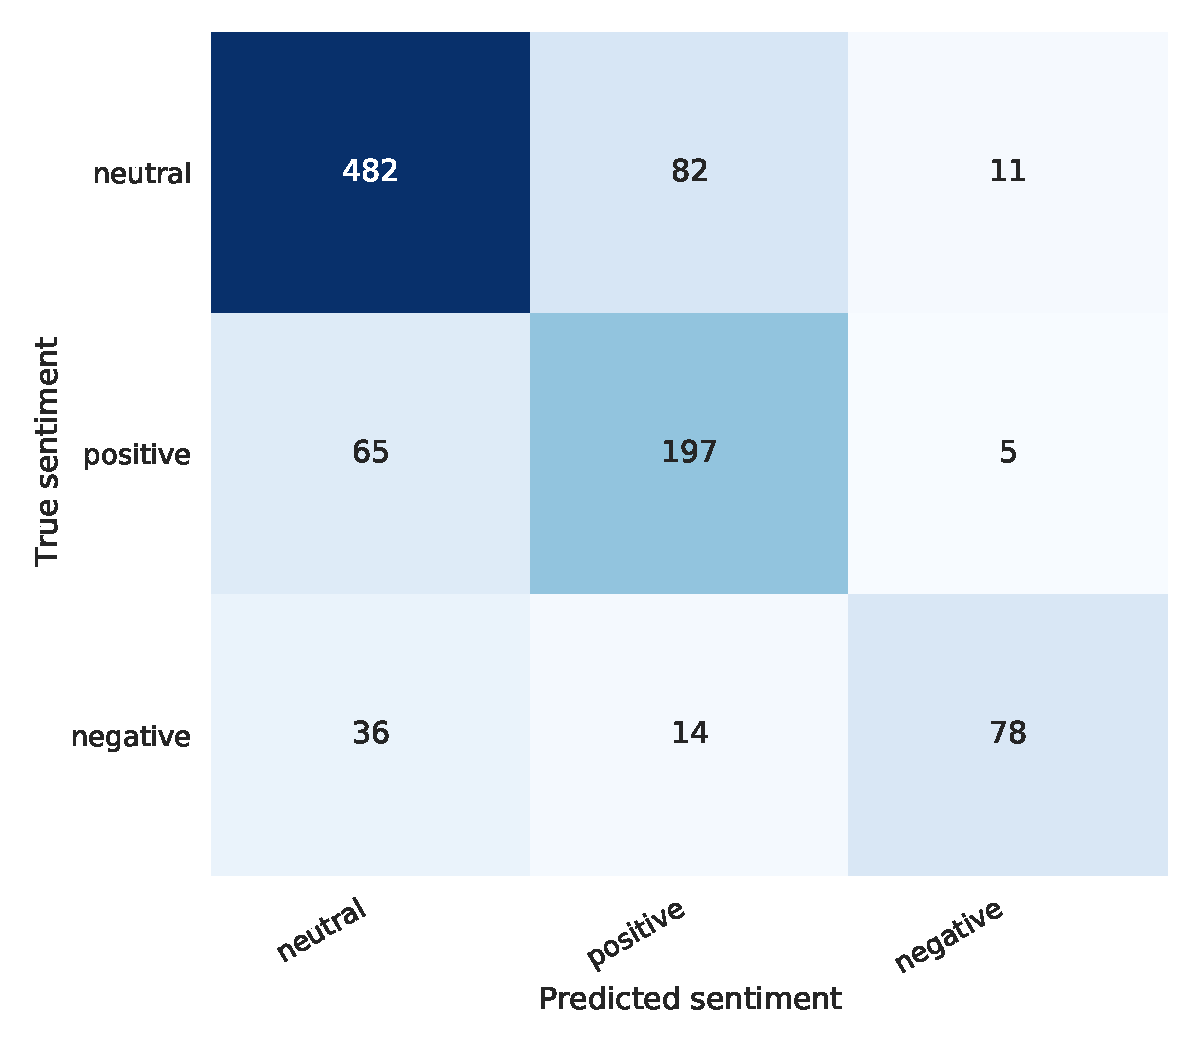
\includegraphics[width=6.3cm]{fig/GRU_cm.pdf}
		\vspace{-0.1\baselineskip}
		\caption{\centering GRU}
	\end{subfigure}
	\par\medskip
	\begin{subfigure}[t]{\linewidth}
		\centering\captionsetup{width=\linewidth}
		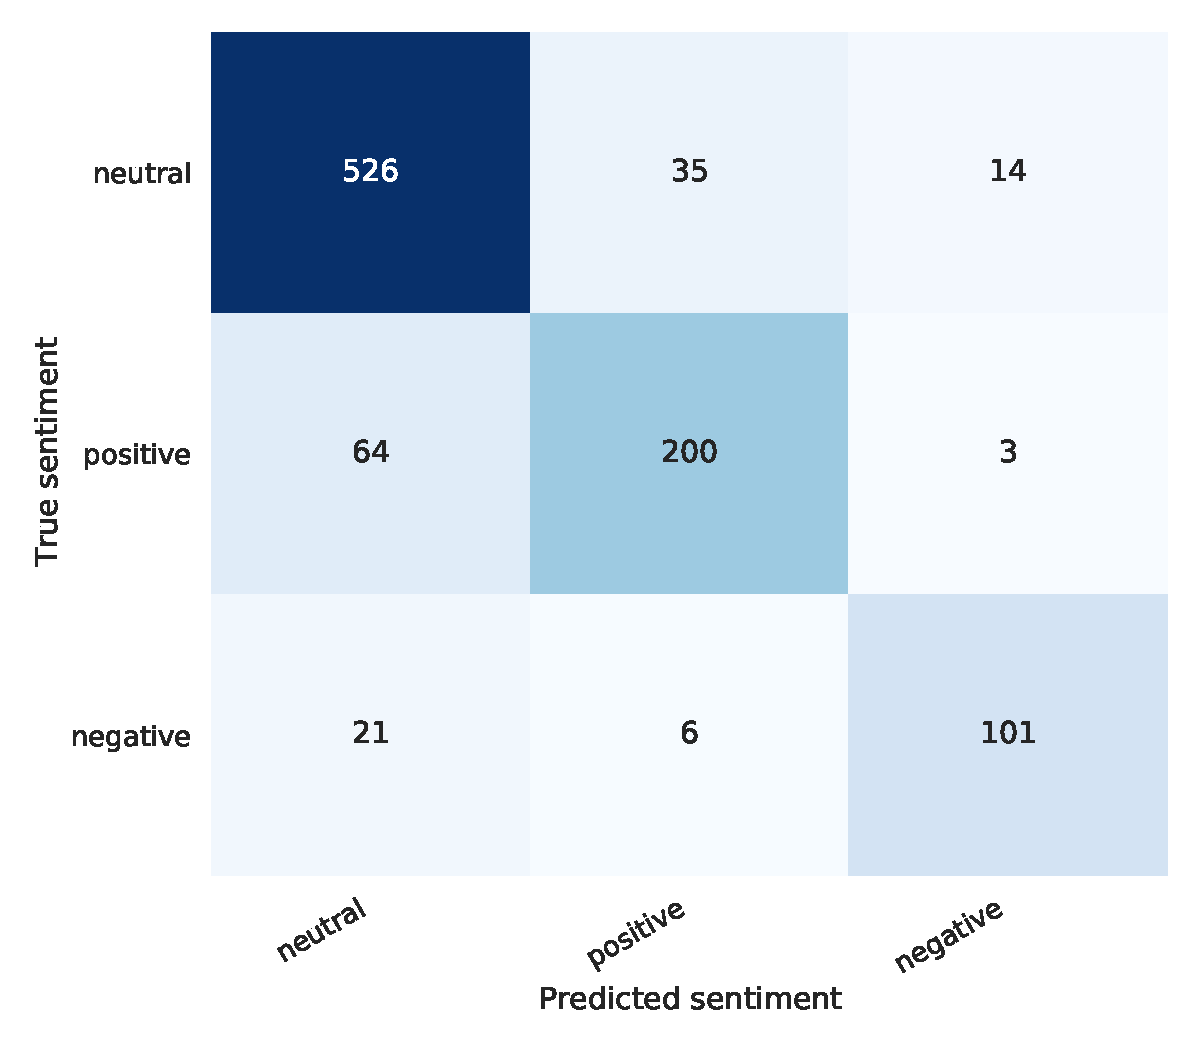
\includegraphics[width=6.3cm]{fig/BERT_cm.pdf}
		\vspace{-0.1\baselineskip}
		\caption{\centering BERT}
	\end{subfigure}\hfill
	\caption{\centering Confusion Matrices of the Best Performing GRU (a) and BERT (b) Models on the Held-out Test Set}
	\label{fig:cms}
\end{figure}



\section{Conclusion}

This project presents a comprehensive study of NLP-based methods for sentiment analysis in finance. It begins with a word counting based approach, explores word encoders and concludes with Transformers, which are at the core of the on-going revolution in the domain. Transformers show superior performances compared to the other evaluated approaches. An important take away is that text representation methods, which feed the semantic meaning of words and sentences into the models, play a central role in sentiment analysis.\\
\\
The financial domain is characterized by a domain-specific language, which adds to the difficulty of financial sentiment analysis. This aspect, which is not covered in this project, is an important topic of research for anyone looking to get improved performances. Even though generic (pre-trained) sentiment analysis models produce decent results, they probably lose some of their effectiveness when applied to specific domains such as finance. Further pre-training on a financial corpus (e.g. in the masked language model setting) and fine-tuning for sentiment analysis, as explored in \cite{FinBERT}, could lead to improved results.\\
\\
Being completely new to natual language processing, this project was an opportunity to get familiar with the various popular methods used to process sequential data. With hindsight, I have developed a good understanding of some of the key concepts used in NLP research nowadays.

{\small
	\bibliographystyle{unsrt}
	\bibliography{egbib}
}

\end{document}

https://ieeexplore.ieee.org/document/9142175